\documentclass{beamer}

% 编码相关.
\usepackage[utf8]{inputenc} % 字符编码.
\usepackage{ctex} % 支持中文.
\usepackage{color, xcolor} % 颜色.

% 目录标题引用.
% \usepackage[hidelinks]{hyperref} % 超链接[colorlinks, linkcolor=red, anchorcolor=blue, citecolor=green]
% \usepackage{cite} % 参考文献.
% \usepackage{appendix} % 附录.

% 排版相关.
\usepackage{multicol} % 多列排版.
\usepackage{fancyhdr} % 页眉页脚.
\usepackage{listings} % 代码环境.
\usepackage{graphicx, subfig} % 插图.
\usepackage{float} % 浮动位置.
\usepackage{enumerate} % 编号itemize.

% 数学环境.
\usepackage{amsfonts} % mathbb, mathfrak.
\usepackage{eucal} % mathcal命令是欧拉书写体, mathscr.
\usepackage{amsmath} % 定义多行公式环境和一系列排版数学公式的命令, 例如连分数\cfrac.
\usepackage{amssymb} % 它定义了amsfonts宏包里msam和mabm字库中全部数学符号的命令.
\usepackage{gensymb} % 数学符号补充.
\usepackage{amsthm} % 定义proof环境, 能自动添加证毕符号, \newtheorem{定理环境名}{标题}[计数器名].
\usepackage[ruled]{algorithm2e} % 算法环境包
\usepackage{tikz} % 绘图.
\usetikzlibrary{positioning}

\title{三角形网格的殷集修补算法}
\author{王则豫}
\institute{浙江大学数学科学学院}
\date{\today}

\usetheme{Madrid}
\usecolortheme{default}
\setbeamertemplate{navigation symbols}{}

\begin{document}

\frame{\titlepage}

\begin{frame}{目录}
    \tableofcontents
\end{frame}

\section{section}
\begin{frame}{title}
    \begin{columns}
        \column{0.45\textwidth}
        \begin{figure}
            \includegraphics[width=0.8\textwidth]{figure.png}
            \caption{caption}
        \end{figure}
        \column{0.45\textwidth}
        \begin{figure}
            \includegraphics[width=0.8\textwidth]{figure.png}
            \caption{caption}
        \end{figure}
    \end{columns}
\end{frame}

\begin{frame}{title}
    \begin{columns}
        \column{0.3\textwidth}
        \begin{figure}
            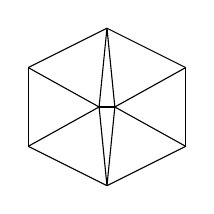
\begin{tikzpicture}
            \draw [black](1,0.5)--(1,-0.5);
            \draw [black](1,0.5)--(0,1);
            \draw [black](0,1)--(-1,0.5);
            \draw [black](-1,0.5)--(-1,-0.5);
            \draw [black](-1,-0.5)--(0,-1);
            \draw [black](0,-1)--(1,-0.5);
            \draw [black](0.1,0)--(0,1);
            \draw [black](0.1,0)--(0,-1);
            \draw [black](0.1,0)--(1,0.5);
            \draw [black](0.1,0)--(1,-0.5);
            \draw [black](-0.1,0)--(0,1);
            \draw [black](-0.1,0)--(0,-1);
            \draw [black](-0.1,0)--(-1,0.5);
            \draw [black](-0.1,0)--(-1,-0.5);
            \draw [black](-0.1,0)--(0.1,0);
            \end{tikzpicture}
            \caption{边长过短}
        \end{figure}
        \column{0.3\textwidth}
        \begin{figure}
            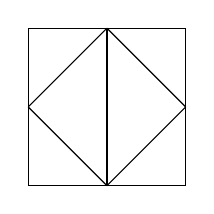
\begin{tikzpicture}
            \draw [black](1,1)--(1,-1);
            \draw [black](1,-1)--(-1,-1);
            \draw [black](-1,-1)--(-1,1);
            \draw [black](-1,1)--(1,1);
            \draw [black](0,1)--(0,-1);
            \draw [black](0,1)--(1,0);
            \draw [black](0,1)--(-1,0);
            \draw [black](0,-1)--(1,0);
            \draw [black](0,-1)--(-1,0);
            \end{tikzpicture}
            \caption{边长过长}
        \end{figure}
        \column{0.3\textwidth}
        \begin{figure}
            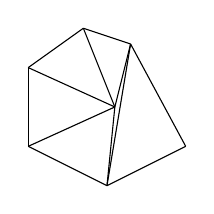
\begin{tikzpicture}
            \draw [black](0.3,0.8)--(1,-0.5);
            \draw [black](0.3,0.8)--(-0.3,1);
            \draw [black](-0.3,1)--(-1,0.5);
            \draw [black](-1,0.5)--(-1,-0.5);
            \draw [black](-1,-0.5)--(0,-1);
            \draw [black](0,-1)--(1,-0.5);
            \draw [black](0.1,0)--(-0.3,1);
            \draw [black](0.1,0)--(0,-1);
            \draw [black](0.1,0)--(-1,0.5);
            \draw [black](0.1,0)--(-1,-0.5);
            \draw [black](0.1,0)--(0.3,0.8);
            \draw [black](0,-1)--(0.3,0.8);
            \end{tikzpicture}
            \caption{内角过小}
        \end{figure}
    \end{columns}
\end{frame}

\begin{frame}{}

\centering \Huge
\emph{请各位老师同学批评指正!}

\end{frame}

\end{document}